\subsection{Convolutional Neural Networks}

Convolutional Neural Network (CNN) \cite{lecun1995convolutional, lecun1989backpropagation} are the type of Neural Networks with at least one convolutional layer. The first convolutional neural networks were LeNet \cite{cnnLecun1998} and AlexNet \cite{krizhevsky2012imagenet}, using only a few convolutional layers. CNNs are assuming that the input data consists of hierarchical patterns which can be used instead of relying on individual features and creating a connection between every single feature and neuron. This approach helps to reduce the number of parameters required by the network.

\subsubsection*{Convolutional Layer}

The convolutional layer uses the idea of filters/kernels with a given size and depth. A layer like that produces the output called a feature map, which is a combination of all the outputs from the kernels. As mentioned, each kernel is defined by the size (which corresponds to its width and height), depths (usually the depth of the input), and additional parameters like padding, stride, or dilatation. The name "convolutional" comes from the mathematical operation of convolution, which is denoted by $f*g$, and the output of that operation is a function that described how one function modifies the other. It can be defined as:

\begin{equation}
    g(m,n) = (h*f)(m,n) = \sum_{u} \sum_{v} h(u,v)f(m-u,n-v)
\end{equation}

Where $f$ is the input image, $h$ is the kernel, $m$ and $n$ are the corresponding row and column in the feature map, and $u$ and $v$ range over all legal subscripts for $h(u,v)$ and $f(m-u,n-v)$ \cite{keller2010convolutions}. An example of the convolution operation for the $m=0, n=3$ is shown in Figure \ref{fig:convolutional operation}.

\begin{figure}[ht]
    \centering
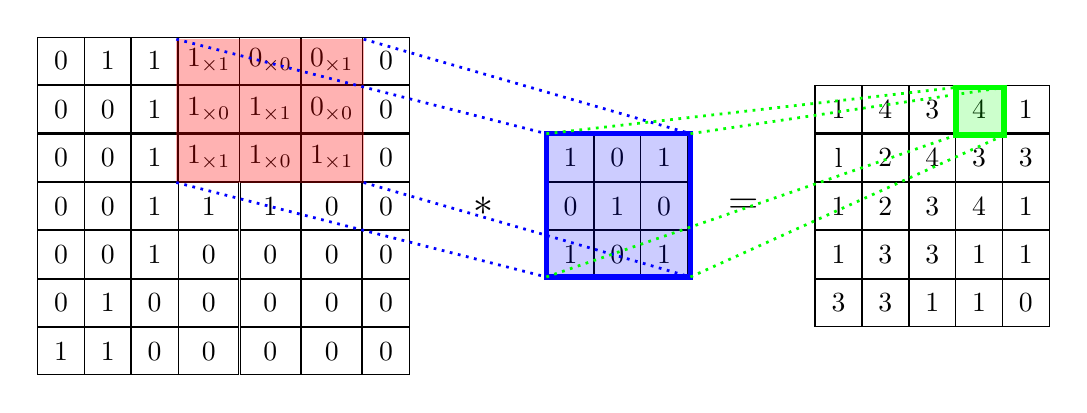
\begin{tikzpicture}[scale=1.0]

  \matrix [nodes=draw,column sep=-0.2mm, minimum size=6mm]
  {
    \node {0}; & \node{1}; & \node {1}; & \node{$1_{\times 1}$}; & \node{$0_{\times 0}$}; 
    & \node{$0_{\times 1}$}; & \node{0}; \\
    \node {0}; & \node{0}; & \node {1}; & \node{$1_{\times 0}$}; & \node{$1_{\times 1}$}; 
    & \node{$0_{\times 0}$}; & \node{0}; \\
    \node {0}; & \node{0}; & \node {1}; & \node{$1_{\times 1}$}; & \node{$1_{\times 0}$}; 
    & \node{$1_{\times 1}$}; & \node{0}; \\
    \node {0}; & \node{0}; & \node {1}; & \node{\, 1 \,}; & \node{\, 1 \, }; 
    & \node{\, 0 \,}; & \node{0}; \\
    \node {0}; & \node{0}; & \node {1}; & \node{\, 0 \, }; & \node{\, 0 \, }; 
    & \node{\, 0 \,}; & \node{0}; \\
    \node {0}; & \node{1}; & \node {0}; & \node{\, 0 \, }; & \node{\, 0 \, }; 
    & \node{\, 0 \,}; & \node{0}; \\
    \node {1}; & \node{1}; & \node {0}; & \node{\, 0 \,}; & \node{\, 0 \, }; 
    & \node{\, 0 \,}; & \node{0}; \\
  };


  % coordinates for coloring filter in array
  \coordinate (A) at (-0.6,0.3);
  \coordinate (B) at (1.78,0.3);
  \coordinate (C) at (1.78,2.12);
  \coordinate (D) at (-0.6,2.12);
  \fill[red, opacity=0.3] (A)--(B)--(C)--(D)--cycle;
  \begin{scope}[shift={(3.3,0)}]
    \node[] at (0,0) {\Large $\ast$};
  \end{scope}[shift={(2.5,0)}]

  \begin{scope}[shift={(5,0)}]

    %\matrix [matrix of math nodes,left delimiter={[},right
    %delimiter={]}]
    \matrix [nodes=draw,column sep=-0.2mm, minimum size=6mm]
    {
      \node{1};  & \node{0};   & \node{1};  \\
      \node{0};  & \node{1};   & \node{0};  \\
      \node{1}; & \node{0}; & \node{1}; \\
    };
    \coordinate (A1) at (-0.9,-0.9);
    \coordinate (B1) at (0.93,-0.9);
    \coordinate (C1) at (0.93,0.92);
    \coordinate (D1) at (-0.9,0.92);
    \fill[blue, opacity=0.2] (A1)--(B1)--(C1)--(D1)--cycle;
    \draw[blue, line width=2] (A1)--(B1)--(C1)--(D1)--cycle;
  \end{scope}

  \draw[dotted, line width=1, color=blue] (A)--(A1);
  \draw[dotted, line width=1, color=blue] (B)--(B1);
  \draw[dotted, line width=1, color=blue] (C)--(C1);
  \draw[dotted, line width=1, color=blue] (D)--(D1);

  \begin{scope}[shift={(6.6,0)}]
    \node[] at (0,0) {\Large $=$};
  \end{scope}[shift={(2.5,0)}]

  \begin{scope}[shift={(9,0)}]

    %\matrix [matrix of math nodes,left delimiter={[},right
    %delimiter={]}]
    \matrix [nodes=draw,column sep=-0.2mm, minimum size=6mm]
    {
      \node{1};  & \node{4};   & \node{3}; & \node{4}; & \node{1};  \\
      \node{l};  & \node{2};   & \node{4}; & \node{3}; & \node{3};  \\
      \node{1}; & \node{2}; & \node{3}; & \node{4} ; & \node{1};  \\
      \node{1}; & \node{3}; & \node{3}; & \node{1} ; & \node{1};  \\
      \node{3}; & \node{3}; & \node{1}; & \node{1} ; & \node{0};  \\
    };
    \coordinate (A2) at (0.3,0.9);
    \coordinate (B2) at (0.91,0.9);
    \coordinate (C2) at (0.91,1.507);
    \coordinate (D2) at (0.3,1.507);
    \fill[green, opacity=0.2] (A2)--(B2)--(C2)--(D2)--cycle;
    \draw[green, line width=2] (A2)--(B2)--(C2)--(D2)--cycle;
  \end{scope}

  \draw[dotted, line width=1, color=green] (A1)--(A2);
  \draw[dotted, line width=1, color=green] (B1)--(B2);
  \draw[dotted, line width=1, color=green] (C1)--(C2);
  \draw[dotted, line width=1, color=green] (D1)--(D2);
\end{tikzpicture}
    \caption{Example of the convolutional operation}
    \label{fig:convolutional operation}
\end{figure}

The standard convolutional layer uses multiple kernels at once, and every one of them has $\text{size} \times \text{size}$ learnable parameters. Putting that in a context where a fully connected neural network requires a weight for every pixel of the input image times the number of neurons in the hidden layer, a convolutional layer is a huge decrease in the total number of parameters. A kernel with a size of $3$ has $9$ learnable parameters. Even with having 50 kernels in the convolutional layer, there are only $450$ learnable parameters in total (for any input image size). For a $32\times32$ image, a fully connected layer with 10 neurons would require $10240$ parameters. It is worth noticing that kernels do not have to be square. The square is computationally efficient, but there were tries to use different shapes \cite{luo2019hexagonal, graham2015sparse, thomas2019kpconv}.

\subsubsection*{Pooling Layer}

CNNs have an additional type of layer called the \textit{Pooling Layer}. There are two types of pooling layers called: \textit{Max Pooling} and \textit{Average Pooling}. Each pooling layer is defined by its size (called the window size), and the result is based only on pixels from that window. The value returned by the max pooling layer is the maximum value from the window. The average pooling layer returns the average from all values from that window.

\begin{figure}[ht]
    \centering
    \begin{subfigure}{.49\textwidth}
        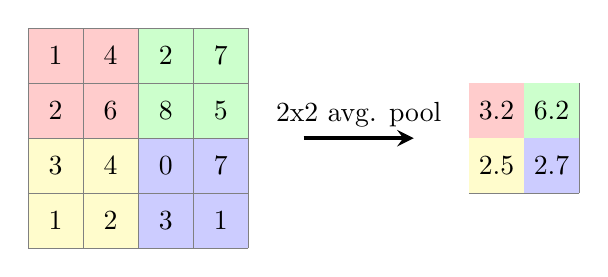
\begin{tikzpicture}[scale=0.7]
        \fill[yellow!20] (0,0) rectangle (2,2);
        \fill[red!20] (0,2) rectangle (2,4);
        \fill[green!20] (2,2) rectangle (4,4);
        \fill[blue!20] (2,2) rectangle (4,0);
        %...
        \draw[gray,very thin] (0,0) grid (4,4);
        \node at (0.5,0.5) {1};
        \node at (1.5,0.5) {2};
        \node at (2.5,0.5) {3};
        \node at (3.5,0.5) {1};
        \node at (0.5,1.5) {3};
        \node at (1.5,1.5) {4};
        \node at (2.5,1.5) {0};
        \node at (3.5,1.5) {7};
        \node at (0.5,2.5) {2};
        \node at (1.5,2.5) {6};
        \node at (2.5,2.5) {8};
        \node at (3.5,2.5) {5};
        \node at (0.5,3.5) {1};
        \node at (1.5,3.5) {4};
        \node at (2.5,3.5) {2};
        \node at (3.5,3.5) {7};
        %...
        \draw[-stealth,ultra thick] (5,2) --node[above] { 2x2 avg. pool} (7,2);
        \draw[gray,very thin] (8,1) grid (10,3);
        \fill[yellow!20] (8,1) rectangle (9,2);
        \fill[red!20] (8,2) rectangle (9,3);
        \fill[green!20] (9,2) rectangle (10,3);
        \fill[blue!20] (9,1) rectangle (10,2);
        \node at (8.5,1.5) {2.5};
        \node at (9.5,1.5) {2.7};
        \node at (8.5,2.5) {3.2};
        \node at (9.5,2.5) {6.2};
        
        \end{tikzpicture}
    \caption{Average Pooling}
    \label{fig:cnn-avg-pooling}
    \end{subfigure}
    \begin{subfigure}{.49\textwidth}
        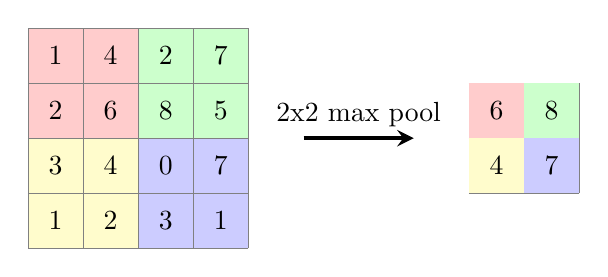
\begin{tikzpicture}[scale=0.7]
        \fill[yellow!20] (0,0) rectangle (2,2);
        \fill[red!20] (0,2) rectangle (2,4);
        \fill[green!20] (2,2) rectangle (4,4);
        \fill[blue!20] (2,2) rectangle (4,0);
        %...
        \draw[gray,very thin] (0,0) grid (4,4);
        \node at (0.5,0.5) {1};
        \node at (1.5,0.5) {2};
        \node at (2.5,0.5) {3};
        \node at (3.5,0.5) {1};
        \node at (0.5,1.5) {3};
        \node at (1.5,1.5) {4};
        \node at (2.5,1.5) {0};
        \node at (3.5,1.5) {7};
        \node at (0.5,2.5) {2};
        \node at (1.5,2.5) {6};
        \node at (2.5,2.5) {8};
        \node at (3.5,2.5) {5};
        \node at (0.5,3.5) {1};
        \node at (1.5,3.5) {4};
        \node at (2.5,3.5) {2};
        \node at (3.5,3.5) {7};
        %...
        \draw[-stealth,ultra thick] (5,2) --node[above] { 2x2 max pool} (7,2);
        \draw[gray,very thin] (8,1) grid (10,3);
        \fill[yellow!20] (8,1) rectangle (9,2);
        \fill[red!20] (8,2) rectangle (9,3);
        \fill[green!20] (9,2) rectangle (10,3);
        \fill[blue!20] (9,1) rectangle (10,2);
        \node at (8.5,1.5) {4};
        \node at (9.5,1.5) {7};
        \node at (8.5,2.5) {6};
        \node at (9.5,2.5) {8};
        
        \end{tikzpicture}
    \caption{Max Pooling}
    \label{fig:cnn-max-pooling}
    \end{subfigure}
    \caption{Example of pooling layers results applied to the same $4 \times 4$ feature map. Colors indicate the area from which the values are pulled to produce the result.}
    \label{fig:cnn-pooling}
\end{figure}